%%%%%%%%%%%%%%%%%%%%%%%%%%%%%%%%%%%%%%%%%%%%%%%%%%%%%%%%%%%%%%%%%%%%%%
% BAB METODOLOGI
%=====================================================================
\renewcommand{\thechapter}{\Roman{chapter}}
\addtocontents{toc}{\vskip10pt}
\chapter{METODOLOGI}
\renewcommand{\thechapter}{\arabic{chapter}}
%---------------------------------------------------------------------

%---------------------------------------------------------------------

%=====================================================================
\section{Diagram Alir Penelitian}
%=====================================================================

Dalam konteks penelitian ini, penting untuk menyadari bahwa pencapaian hasil yang berkualitas dan signifikan melibatkan proses yang terstruktur dan sistematis. Progres yang efektif dalam eksplorasi masalah penelitian didasarkan pada langkah-langkah yang diatur secara terencana dan berkesinambungan. Oleh karena itu, penelitian ini menjelaskan dan mengikuti serangkaian tahapan yang saling terkait, yang dirinci secara kronologis dan terurai dalam diagram alir yang dapat dilihat pada Gambar 3.1. \begin{figure}
    \centering
    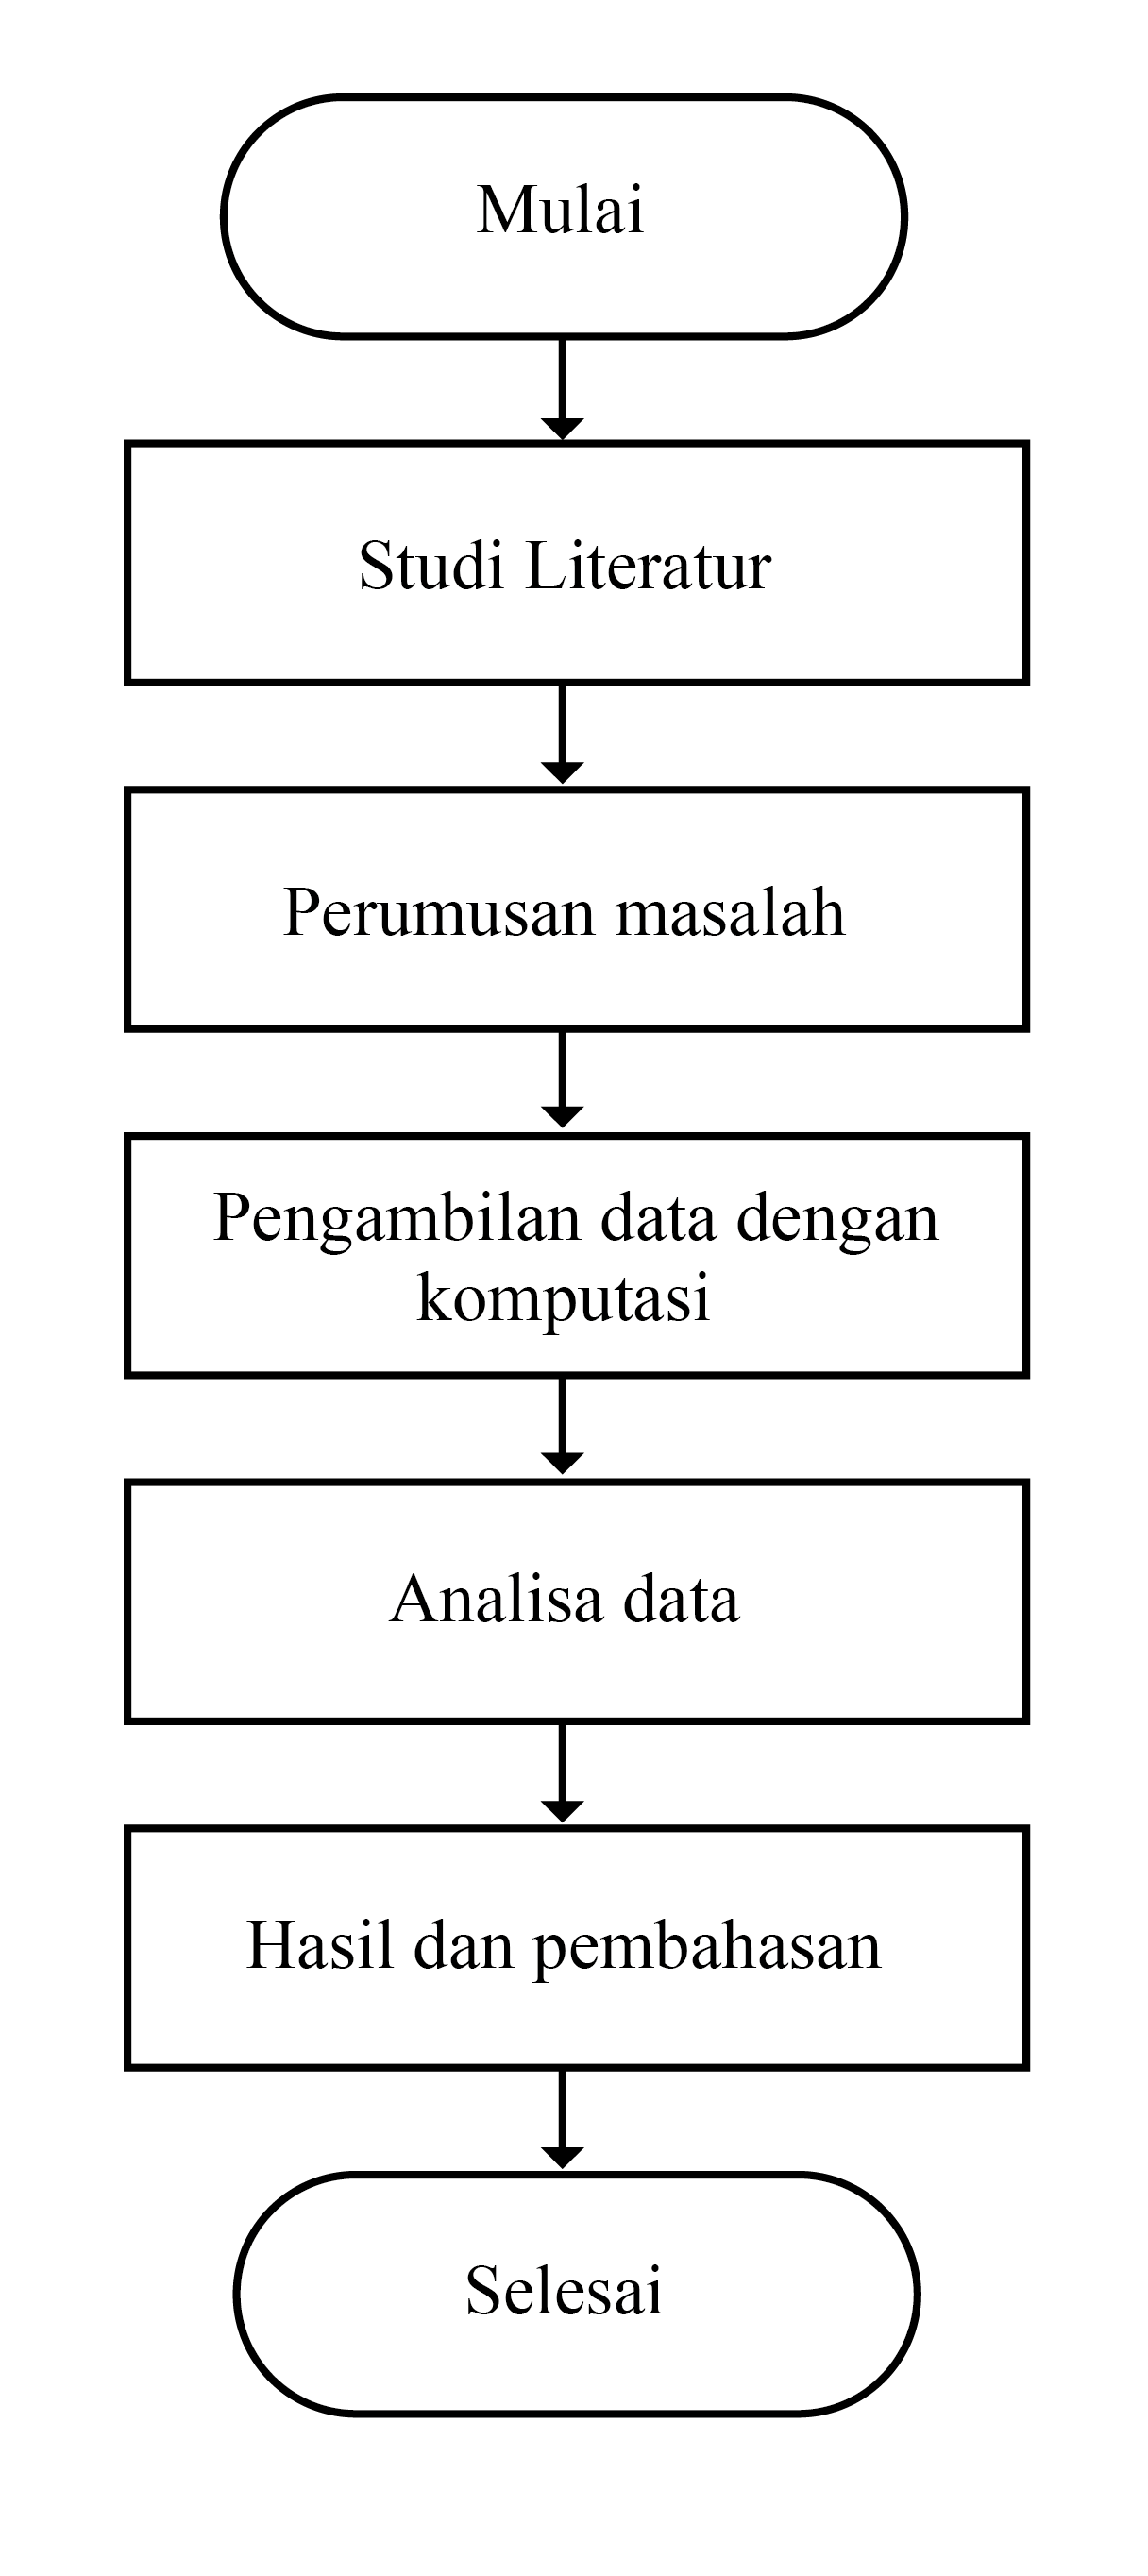
\includegraphics[width=5cm]{gambar/Flowchart Kegiatan.png}
    \caption{Diagram Alir Penelitian}
\end{figure}

%=====================================================================
\section{Jenis dan Desain Penelitian}
%=====================================================================
Pada penelitian ini, jenis penelitian yang digunakan adalah penelitian komputasi, yaitu penelitian yang dilakukan di dalam komputer dengan metode pemodelan mekanika dinamika molekular (MD) dan \textit{ab-initio calculation} untuk menyelidiki sifat elektronik pada struktur material Boron Nitride Heksagonal (hBN) akibat pengaruh suhu menggunakan perangkat lunak LAMMPS dan Quantum ESPRESSO. \section{Rencana Penelitian }

Penelitian ini bertujuan untuk mempelajari sifat elektronik dan magnetik dari hBN sheet 2D single layer dengan dimensi 4x4x1. Struktur hBN disiapkan dan divalidasi melalui studi literatur serta simulasi awal. Selanjutnya, struktur dipanaskan menggunakan LAMMPS guna mencapai kondisi termal optimal, dan hasil pemanasan dianalisis dengan Quantum ESPRESSO untuk mendapatkan informasi mengenai perubahan sifat elektroniknya. Berikut adalah rencana kegiatan penelitian yang berlangsung selama 6 bulan:

\bigskip

\begin{figure}[htbp]
\centering  
\begin{ganttchart}[
    hgrid,
    vgrid,
    title height=1,
    x unit =1cm,
    bar/.style={fill=blue!50},
    milestone/.style={fill=red}
]{1}{6}  % Skala waktu: bulan 1 sampai 6
  % Baris judul untuk bulan
  \gantttitle{\textbf{Bulan}}{6} \\
  \gantttitle{\mbox{Jan}}{1}
  \gantttitle{\mbox{Feb}}{1}
  \gantttitle{\mbox{Mar}}{1}
  \gantttitle{\mbox{Apr}}{1}
  \gantttitle{\mbox{Mei}}{1}
  \gantttitle{\mbox{Jun}}{1} \\
  % Kegiatan penelitian
  \ganttbar{Studi Literatur \& Persiapan Model}{1}{1} \\
  \ganttbar{Persiapan Proposal}{1}{2}\\
  \ganttbar{Simulasi Pemanasan (LAMMPS)}{2}{3} \\
  \ganttbar{Pengumpulan Proposal}{3}{3}\\
  \ganttbar{Analisis Struktur (Quantum ESPRESSO)}{4}{4} \\
  \ganttbar{Penyusunan Laporan}{5}{5} 
 \\
  \ganttbar{Revisi dan Finalisasi Laporan}{6}{6}
\end{ganttchart}
\caption{Gantt Chart Rencana Penelitian Sifat Elektronik hBN Sheet 2D.}
\label{fig:gantt}
\end{figure}

\bigskip

%---------------------------------------------------------------------
\section{Perangkat Penelitian}
%---------------------------------------------------------------------
Dalam prosedur penelitian ini, kami secara komprehensif membahas perangkat dan metodologi yang digunakan untuk menganalisis sifat elektronik lembaran \textit{hexagonal boron nitride} (hBN) 2D yang telah dipanaskan. Penelitian ini dilakukan melalui dua tahap utama, yaitu simulasi dinamika molekul (MD) menggunakan LAMMPS untuk memodelkan evolusi struktur hBN pada rentang suhu 500K hingga 4000K, serta perhitungan teori fungsional kerapatan (DFT) menggunakan Quantum ESPRESSO untuk mengevaluasi perubahan sifat elektronik setelah pemanasan. Pada tahap awal, kami memberikan gambaran tentang perangkat keras dan perangkat lunak yang digunakan, termasuk spesifikasi sistem komputasi berperforma tinggi yang mendukung simulasi dan analisis data. Proses pembuatan dan optimasi struktur hBN dilakukan dengan \textit{Atomic Simulation Environment} (ASE), diikuti dengan simulasi pemanasan menggunakan potensial ReaxFF dalam LAMMPS. Selama simulasi MD, parameter seperti \textit{Radial Distribution Function} (RDF) dan \textit{Mean Squared Displacement} (MSD) dikumpulkan untuk memantau perubahan struktur dan dinamika atom. Setelah simulasi MD, struktur akhir dikonversi ke format yang kompatibel dengan Quantum ESPRESSO untuk perhitungan DFT lebih lanjut. Proses ini melibatkan perhitungan \textit{Self-Consistent Field} (SCF) untuk mendapatkan kerapatan muatan yang stabil, diikuti dengan \textit{Non-Self-Consistent Field} (NSCF) untuk menghitung struktur pita elektronik, \textit{Density of States} (DOS), \textit{Projected Density of States} (PDOS), serta distribusi muatan (\textit{charge density}). Seluruh perhitungan dilakukan dengan pendekatan spin-polarized menggunakan fungsi pertukaran-korelasi PBEsol PAW. Untuk memahami perubahan sifat elektronik akibat pemanasan, hasil perhitungan DFT divisualisasikan dan dianalisis menggunakan OVITO, VMD, XCrySDen, dan VESTA, sementara pemrosesan data numerik dilakukan dengan NumPy, Matplotlib, dan Seaborn. Dengan dokumentasi prosedur yang jelas dan parameter yang terperinci, penelitian ini diharapkan dapat memberikan wawasan mendalam tentang pengaruh suhu terhadap sifat elektronik hBN serta memungkinkan replikasi dan validasi oleh penelitian lain. \section{Perangkat Penelitian}
Dalam penelitian ini, perangkat penelitian terdiri dari perangkat keras dan perangkat lunak yang digunakan untuk mendukung simulasi dan analisis sifat elektronik dari struktur lembaran \textit{hexagonal boron nitride} (hBN) 2D setelah pemanasan. Kombinasi perangkat keras berperforma tinggi dan perangkat lunak komputasi canggih memungkinkan penelitian ini dilakukan secara efisien dan akurat. \subsection{Perangkat Keras}
Penelitian ini dilakukan pada sistem komputasi dengan spesifikasi sebagai berikut:
\begin{enumerate}
    \item 3 node komputasi. \item Setiap node memiliki 1x AMD EPYC 7702P, dengan 64 core / 128 thread, kecepatan 2.0 GHz. \item RAM sebesar 240 GB.
    \item Interkoneksi menggunakan Mellanox RoCE 100Gbps. \end{enumerate}

\subsection{Perangkat Lunak}
Penelitian ini menggunakan berbagai perangkat lunak untuk mendukung simulasi dan analisis data. Quantum ESPRESSO digunakan sebagai perangkat lunak utama dalam perhitungan DFT, memungkinkan evaluasi struktur elektronik material dengan pendekatan \textit{plane-wave pseudopotential}. LAMMPS digunakan untuk simulasi dinamika molekul (MD), di mana interaksi antar-atom dimodelkan menggunakan potensial ReaxFF untuk memahami efek pemanasan pada struktur hBN. Untuk visualisasi hasil simulasi dan analisis struktur, berbagai perangkat lunak digunakan, termasuk VMD, OVITO, XCrySDen, dan VESTA. VMD digunakan untuk menampilkan dinamika atom secara real-time dalam simulasi MD, sementara OVITO menyediakan alat analisis struktur kristal yang lebih fleksibel. XCrySDen membantu dalam visualisasi struktur elektronik dari hasil perhitungan Quantum ESPRESSO, dan VESTA digunakan untuk menampilkan distribusi kerapatan muatan serta struktur pita elektronik. Pembuatan dan manipulasi struktur kristal dilakukan menggunakan \textit{Atomic Simulation Environment} (ASE), yang memungkinkan konversi format dan pembuatan model supercell. Untuk analisis dan pemrosesan data numerik, NumPy digunakan sebagai pustaka utama untuk komputasi numerik, sedangkan Matplotlib dan Seaborn digunakan untuk memvisualisasikan hasil analisis seperti \textit{Radial Distribution Function} (RDF), \textit{Mean Squared Displacement} (MSD), serta data dari perhitungan DFT seperti \textit{Density of States} (DOS) dan \textit{Projected Density of States} (PDOS). Seluruh proses analisis dan pengolahan data dilakukan dalam lingkungan Jupyter Notebook untuk kemudahan dokumentasi dan reprodusibilitas penelitian. %---------------------------------------------------------------------
\section{Prosedur Penelitian}
Dalam prosedur penelitian ini, kami secara komprehensif membahas perangkat dan metodologi yang digunakan untuk menganalisis sifat elektronik lembaran \textit{hexagonal boron nitride} (hBN) 2D yang telah dipanaskan. Penelitian ini dilakukan melalui dua tahap utama, yaitu simulasi dinamika molekul (MD) menggunakan LAMMPS untuk memodelkan evolusi struktur hBN pada rentang suhu 500K hingga 4000K, serta perhitungan teori fungsional kerapatan (DFT) menggunakan Quantum ESPRESSO untuk mengevaluasi perubahan sifat elektronik setelah pemanasan. Pada tahap awal, kami memberikan gambaran tentang perangkat keras dan perangkat lunak yang digunakan, termasuk spesifikasi sistem komputasi berperforma tinggi yang mendukung simulasi dan analisis data. Proses pembuatan dan optimasi struktur hBN dilakukan dengan \textit{Atomic Simulation Environment} (ASE), diikuti dengan simulasi pemanasan menggunakan potensial ReaxFF dalam LAMMPS. Selama simulasi MD, parameter seperti \textit{Radial Distribution Function} (RDF) dan \textit{Mean Squared Displacement} (MSD) dianalisis untuk memahami perubahan struktur akibat pemanasan. Setelah simulasi MD, struktur akhir dikonversi ke format yang kompatibel dengan Quantum ESPRESSO untuk perhitungan DFT lebih lanjut. Proses ini melibatkan perhitungan \textit{Self-Consistent Field} (SCF) untuk mendapatkan kerapatan muatan yang stabil, diikuti dengan \textit{Non-Self-Consistent Field} (NSCF) untuk menghitung struktur pita elektronik, \textit{Density of States} (DOS), \textit{Projected Density of States} (PDOS), serta distribusi muatan (\textit{charge density}). Seluruh perhitungan dilakukan dengan pendekatan spin-polarized menggunakan fungsi pertukaran-korelasi PBEsol PAW. Untuk memahami perubahan sifat elektronik akibat pemanasan, hasil perhitungan DFT divisualisasikan dan dianalisis menggunakan OVITO, VMD, XCrySDen, dan VESTA, sementara pemrosesan data numerik dilakukan dengan NumPy, Matplotlib, dan Seaborn. Dengan dokumentasi prosedur yang jelas dan parameter yang terperinci, penelitian ini diharapkan dapat memberikan wawasan mendalam tentang pengaruh suhu terhadap sifat elektronik hBN serta memungkinkan replikasi dan validasi oleh penelitian lain. \vspace{3mm}

\begin{figure}
    \centering
    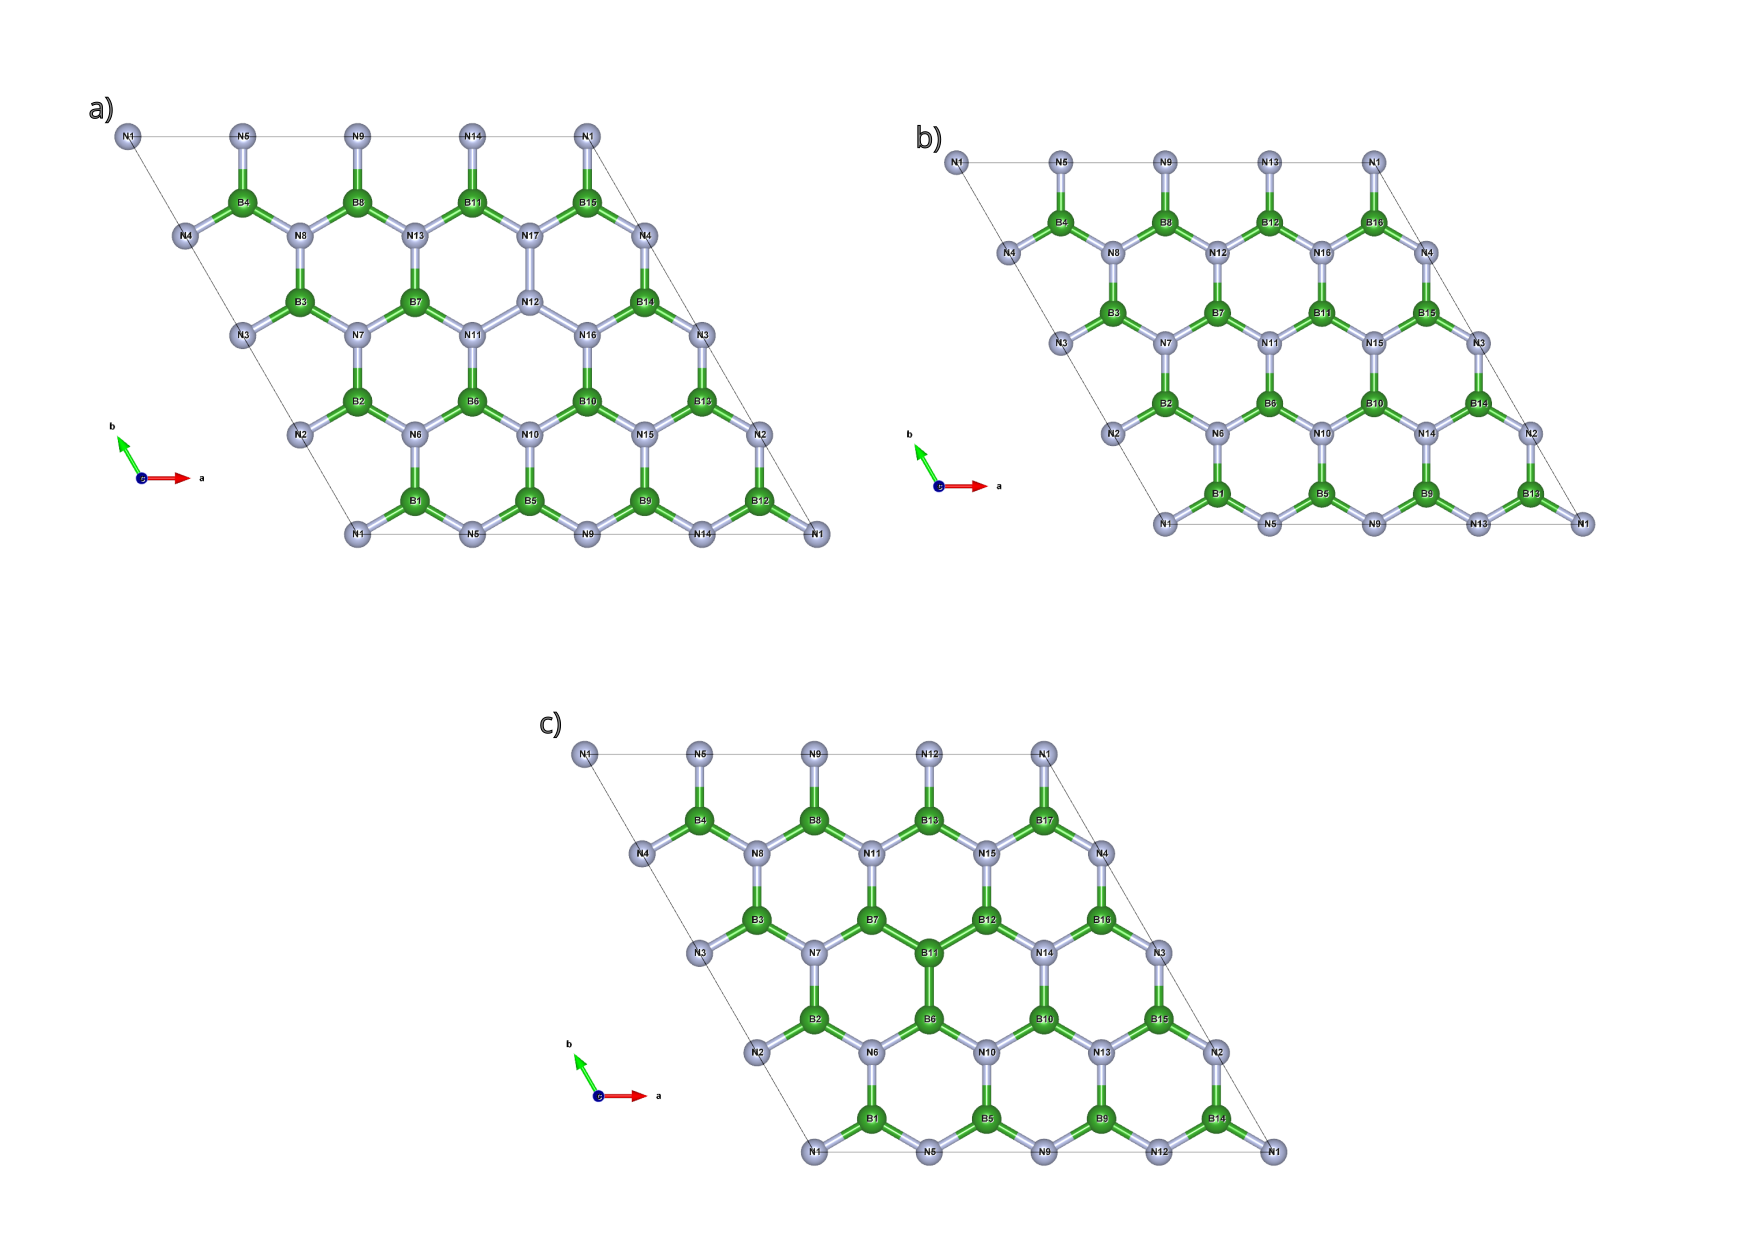
\includegraphics[width=0.8\linewidth]{gambar_hasil/structures_all.png}
    \caption{Model hBN 4x4x1 dengan a) struktur hBN murni b) struktur hBN dengan cacat N-N c) struktur hBN dengan cacat B-B}
    \label{fig:enter-label}
\end{figure}

\subsection{Detail Komputasi}
Dalam penelitian ini digunakan Quantum ESPRESSO \citep{Giannozzi2009} dan LAMMPS \citep{Plimpton1995} sebagai perangkat lunak komputasi. Digunakan supersel 4x4x1 untuk membentuk struktur \textit{hBN} yang dapat dilihat di Gambar 3.3 Kalkulasi dengan LAMMPS menggunakan variasi potensial ReaxFF \citep{Lele2022} dan ensemble NVT dengan pemanasan dari rentang temperatur 500K hingga 4000K. Pada kalkulasi dengan Quantum ESPRESSO digunakan variasi \texttt{ecutwfc} sebesar 60 Ry dan \texttt{K-POINTS} sebesar $8\times8\times1$ untuk membagi daerah Brillouin dengan kisi Monkhorst-Pack (MP) \citep{Monkhorst1976}. Kedua nilai tersebut diperoleh dari uji konvergensi yang akan dijelaskan lebih lengkap pada BAB 4. Digunakan fungsional Perdew-Burke-Ernzerhof (PBE) \citep{Perdew1996} sebagai \textit{generalized gradient approximation} (GGA) untuk melengkapi fungsi korelasi dan pertukaran. Potensial semu yang digunakan untuk menggambarkan elektron valensi dan elektron inti adalah \textit{projector augmented wave method} (PAW) \citep{Blochl1994}. Selain itu, ruang vakum dibuat sebesar 20\AA.
Diagram alir komputasi yang akan dilakukan dalam penelitian ini dapat dilihat pada Gambar 3.5 dan Gambar 3.6. Seluruh prosedur komputasi dalam Gambar 3.5 dilakukan untuk komputasi menggunakan MD sedangkan Gambar 3.6 untuk komputasi menggunakan DFT. Sementara visualisasi data hasil komputasi dibuat dengan bantuan dari kode Python menggunakan library Matplotlib dan NumPy yang dibuat di dalam VS Code dengan Jupyter Notebook. \begin{figure}
    \centering
    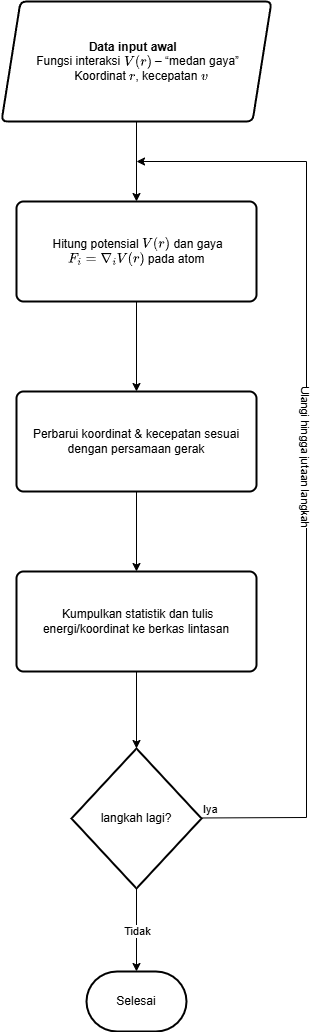
\includegraphics[width=0.35\linewidth]{gambar/MD.drawio.png}
    \caption{Alur Komputasi MD}
    \label{fig:enter-label}
\end{figure}

\begin{figure}
    \centering
    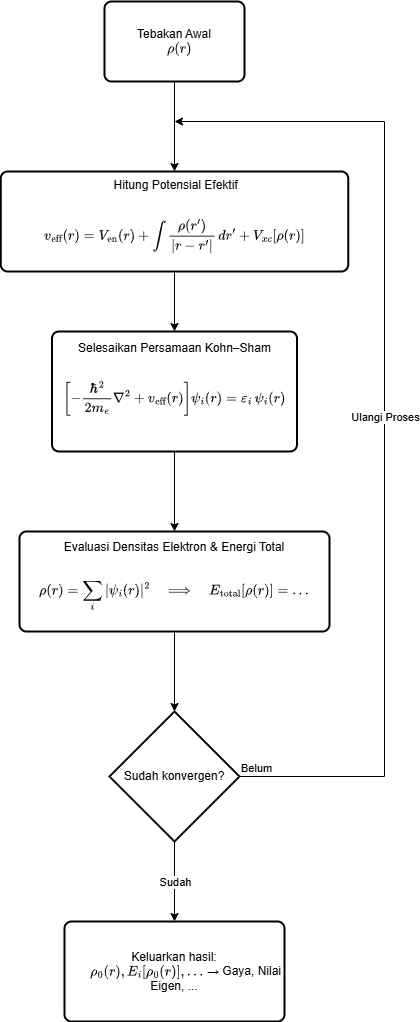
\includegraphics[width=0.5\linewidth]{gambar/DFT.drawio.png}
    \caption{Alur Komputasi DFT }
    \label{fig:enter-label}
\end{figure}

\subsection{Langkah Kerja}
\label{sec:intro}
Penelitian ini bertujuan untuk mengkaji sifat elektronik lembaran \textit{hexagonal boron nitride} (hBN) 2D lapisan tunggal berukuran 4×4×1. Metodologi yang digunakan meliputi simulasi dinamika molekul (MD) dengan LAMMPS dan perhitungan teori fungsional kerapatan (DFT) dengan Quantum ESPRESSO. Visualisasi dan analisis data dilakukan menggunakan OVITO, VMD, XCrySDen, VESTA, serta pustaka Python seperti NumPy, Matplotlib, dan Seaborn. \subsubsection*{Pembuatan dan Relaksasi Struktur Awal hBN}
\label{sec:structure}
\begin{enumerate}
    \item \textbf{Pembuatan Struktur:} Struktur awal hBN 2D lapisan tunggal dengan ukuran 4×4×1 dibuat menggunakan \textit{Atomic Simulation Environment} (ASE). Struktur ini kemudian disimpan dalam format yang kompatibel dengan LAMMPS, seperti file data. \item \textbf{Relaksasi Struktur:} Struktur awal direlaksasi menggunakan LAMMPS dengan potensial ReaxFF khusus untuk hBN. \textit{Time Step} (TS) yang digunakan adalah 0,25 fs. Relaksasi dilakukan hingga gaya antar atom mencapai nilai di bawah 0,01 eV/Å, memastikan struktur berada pada kondisi energi minimum. \end{enumerate}

\subsubsection*{Simulasi Pemanasan dengan MD}
\label{sec:md_simulation}
\begin{enumerate}
    \item \textbf{Proses Pemanasan:} Setelah relaksasi, struktur dipanaskan secara bertahap dari 500K hingga 4000K menggunakan LAMMPS dengan \textit{Time Step} (TS) 0,25 fs. Pemanasan bertahap ini penting untuk menghindari guncangan termal yang dapat menyebabkan ketidakstabilan struktur. \item \textbf{Pengumpulan Data:} Selama simulasi, data seperti \textit{Radial Distribution Function} (RDF) dan \textit{Mean Squared Displacement} (MSD) dikumpulkan untuk memantau perubahan struktur dan dinamika atom. \end{enumerate}

\subsubsection*{Konversi Struktur untuk Perhitungan DFT}
\label{sec:structure_conversion}
Struktur akhir dari simulasi MD diekstraksi dan dikonversi ke format input yang kompatibel dengan Quantum ESPRESSO menggunakan ASE. Konversi ini memastikan tidak ada kehilangan informasi geometri dan gaya residu tetap minimal, sehingga struktur siap untuk perhitungan DFT. \subsubsection*{Perhitungan DFT: SCF dan NSCF}
\label{sec:dft_calculations}
\begin{enumerate}
    \item \textbf{Perhitungan SCF:} Langkah pertama dalam perhitungan DFT adalah melakukan perhitungan \textit{Self-Consistent Field} (SCF) untuk memperoleh distribusi kerapatan muatan yang konsisten dengan potensial yang dihasilkannya. Parameter seperti energi cutoff dan kisi k-point diatur untuk mencapai konvergensi yang baik. \item \textbf{Perhitungan NSCF:} Setelah perhitungan SCF, dilakukan perhitungan \textit{Non-Self-Consistent Field} (NSCF) menggunakan kerapatan muatan yang telah diperoleh. NSCF biasanya dilakukan dengan grid k-point yang lebih rapat atau sepanjang jalur simetri tinggi dalam zona Brillouin. Langkah ini penting untuk menghitung energi eigen secara akurat guna analisis struktur pita dan \textit{Density of States} (DOS). \end{enumerate}

\subsubsection*{Perhitungan Sifat Elektronik dengan Spin Terpolarisasi}
\label{sec:electronic_properties}
Setelah perhitungan NSCF, perhitungan sifat elektronik dilakukan dengan mempertimbangkan polaritas spin. Analisis meliputi:
\begin{enumerate}
    \item \textbf{Struktur Pita (Band Structure, BS):} Menunjukkan hubungan antara energi dan momentum elektron, memberikan informasi tentang sifat konduktif atau isolatif material. \item \textbf{Density of States (DOS):} Menggambarkan jumlah keadaan elektron yang tersedia pada tiap tingkat energi. \item \textbf{Projected Density of States (PDOS):} Menjelaskan kontribusi masing-masing orbital atomik terhadap DOS total. \item \textbf{Kerapatan Muatan (Charge Density):} Menunjukkan distribusi elektron dalam material, penting untuk memahami karakter ikatan kimia.
\end{enumerate}